%% ============================================================================
%%  IEEE Conference Paper (IEEEtran) — generated from the Ens_v2 repository
%%  ----------------------------------------------------------------------------
%%  Compile: pdflatex paper.tex  (twice for cross-references)  |  Overleaf-ready
%%  Class:   IEEEtran [conference]  (standard IEEE conference two-column format)
%%
%%  NOTE FOR AUTHORS: replace the placeholder author block below with real
%%  names / affiliations / e-mails before submission.
%% ============================================================================
\documentclass[conference]{IEEEtran}

% ---- Packages (all standard in TeX Live / Overleaf) -------------------------
\usepackage{cite}            % IEEE-style numeric citations [1]--[3]
\usepackage{amsmath,amssymb,amsfonts}
\usepackage{graphicx}
\usepackage{booktabs}
\usepackage{multirow}
\usepackage{url}
\usepackage{xcolor}
\usepackage{tikz}
\usetikzlibrary{arrows.meta, positioning, fit}
\usepackage[hidelinks]{hyperref}

\hyphenation{prompt-injection}

\begin{document}

% =============================================================================
% Title / Authors  (PLACEHOLDERS — replace before submission)
% =============================================================================
\title{Guardrail Cascades Do Not Compose: Measuring Routing-Induced Starvation in a Three-Layer Prompt-Injection Defense}

\author{\IEEEauthorblockN{First A. Author\IEEEauthorrefmark{1}, Second B. Author\IEEEauthorrefmark{1}}
\IEEEauthorblockA{\IEEEauthorrefmark{1}Department of Computer Science, Example University, City, Country\\
\{first.author, second.author\}@example.edu}
}

\maketitle

% =============================================================================
\begin{abstract}
Prompt injection and jailbreak attacks remain the dominant failure mode for
deployed large language model (LLM) systems, and practitioners increasingly
stack several detectors---a fast surface classifier, a hidden-state probe, and
an output auditor---to defend in depth. The implicit assumption behind such
stacks is that layer-level accuracy \emph{composes}: a stronger component
yields a stronger system. We stress-test this assumption on a three-layer,
fail-closed guardrail wrapped around Qwen2.5-7B-Instruct on two T4 GPUs. In
isolation, our hidden-state probe attains $0.997$ ROC-AUC on a held-out
injection set; yet when routed through a conventional escalation gate that
forwards only ``suspicious'' inputs to the second layer, the full pipeline's
recall ($0.37$) is statistically indistinguishable from that of the surface
classifier alone ($0.35$). The gate silently starved the probe of $38$ of
$60$ held-out injections. Removing the gate---running the second layer
always-on---raises end-to-end recall to $0.90$ at a $1.8\%$ false-positive
rate, at the cost of one additional 7B forward pass (${\sim}50$--$150$~ms) per
request. We formalize why this occurs, show that component-level metrics do not
predict ensemble security, and distill routing-policy recommendations for
layered LLM guardrails. Code, artifacts, and seeds are released for
reproduction on free-tier hardware.
\end{abstract}

\begin{IEEEkeywords}
prompt injection; jailbreak; LLM security; defense in depth; hidden-state
probes; guardrail evaluation; cascade classifiers
\end{IEEEkeywords}

% =============================================================================
\section{Introduction}
\label{sec:intro}

Prompt injection---where an attacker smuggles instructions into the context
window of an LLM to hijack its goal or exfiltrate data---is widely ranked as
the top risk for LLM applications \cite{liu2024}. The attack class spans direct
instruction overrides (\emph{``ignore your previous instructions''})
\cite{perez2022}, indirect injection through retrieved or tool-supplied content
\cite{greshake2023,liu2024}, and jailbreaks that override safety alignment
\cite{zou2023}. Because no single detector is robust to all of these, modern
guardrail practice is defense in depth: a cheap, high-precision surface
classifier screens inputs; a second, more expensive mechanism such as a
hidden-state probe or an LLM-based judge re-examines the remainder; and output
auditors check the response after generation
\cite{inan2023,li2025,injecguard,instructdetector,jbshield}.

Each layer of such a stack is usually developed, benchmarked, and reported
\emph{in isolation}, and the implicit expectation is that a layer with strong
standalone metrics will strengthen the ensemble. In this paper we show that
this expectation can fail in a precisely quantifiable way. We build and release
a three-layer, fail-closed injection guard around Qwen2.5-7B-Instruct
\cite{qwen25}, reproducible on two T4 GPUs, and evaluate it end-to-end on a
held-out injection corpus. The second layer---a logistic probe trained on the
intermediate hidden states of the target LLM---achieves $0.997$ ROC-AUC and
$0.783$ recall \emph{in isolation}. Yet when this probe is placed behind the
standard ``escalation gate'' that only forwards inputs the surface classifier
finds suspicious, the end-to-end recall of the full pipeline ($0.37$) collapses
to that of the surface classifier alone ($0.35$): the gate forwarded only $1$
of $60$ held-out injections to the probe. The probe, despite its near-perfect
AUC, contributed essentially one detection to the ensemble.

This is an instance of a classic principle in cascade design: a cheap first
stage in a cascade must have near-total recall, or every stage behind it is
starved of the very traffic it exists to catch \cite{viola2001}. Our
contribution is not the discovery of this principle, but the demonstration that
production-style LLM guardrail stacks violate it silently, together with a
quantified cost of the violation and a concrete fix. Specifically, we
contribute:

\begin{itemize}
  \item a reproducible, fail-closed three-layer prompt-injection pipeline for
        Qwen2.5-7B-Instruct on two T4 GPUs (surface classifier, hidden-state
        probe, output auditor), released as open source;
  \item a quantified \emph{gate-starvation} result: a component with $0.997$
        AUC contributes a single detection end-to-end because the routing gate
        inherits the surface classifier's blind spots, cutting end-to-end recall
        from the component's $0.78$ to $0.37$;
  \item a minimal, costed fix---always-on routing of the second layer---which
        restores end-to-end recall to $0.90$ at $1.8\%$ FPR for one extra
        7B forward pass per request, together with a threshold operating-point
        analysis; and
  \item routing-policy recommendations and a discussion of the methodological
        traps (small test splits, in-sample threshold calibration, augmentation
        leakage) that hide this failure mode from component-level benchmarks.
\end{itemize}

The remainder of the paper is organized as follows. Section~\ref{sec:related}
reviews related work. Section~\ref{sec:system} describes the pipeline.
Section~\ref{sec:setup} details data, training, and evaluation protocol.
Section~\ref{sec:results} reports results, including the central routing
pathology. Section~\ref{sec:discussion} discusses implications, limitations,
and recommendations, and Section~\ref{sec:conclusion} concludes.

% =============================================================================
\section{Background and Related Work}
\label{sec:related}

\subsection{Threat model}
\label{sec:threat}
We consider a single-turn LLM application that (i) accepts a user instruction,
(ii) optionally augments it with \emph{untrusted} context (retrieved documents,
tool output, web content), and (iii) generates a response under a fixed,
sensitive system prompt. The adversary controls either the user instruction
(direct injection) or the untrusted context (indirect injection), and seeks
goal hijacking or system-prompt exfiltration. This matches the canonical
formulations of Perez and Ribeiro \cite{perez2022} and Greshake et al.
\cite{greshake2023}, and the indirect-injection surface that dominates current
agentic deployments \cite{greshake2023,liu2024}.

\subsection{Detection defenses}
\label{sec:defenses}
Two families of detector dominate practice.

\emph{Surface prompt guards} are lightweight classifiers---typically fine-tuned
DeBERTa-family encoders---that score raw input text. Examples include
prompt guard models trained as binary classifiers, such as PIGuard
\cite{li2025} and InjecGuard \cite{injecguard}, and generative guards such as
Llama Guard \cite{inan2023}. These
models are fast and cheap but are documented to suffer \emph{over-defense}:
bias toward trigger words causes benign inputs stuffed with attack vocabulary to
be misclassified, with accuracy dropping toward chance on adversarial-benign
sets such as NotInject \cite{li2025,injecguard}. We observe the same failure mode in our
first layer, which motivates treating it as a high-precision but
recall-limited stage.

\emph{Representation-level detectors} read the model's internal activations
rather than the surface string. Linear probes on intermediate hidden states have
a long lineage \cite{alain2016} and a growing body of recent work for
injection and jailbreak detection: InstructDetector uses hidden states and
gradients to detect indirect instructions \cite{instructdetector}; JBShield
analyzes activated toxic/jailbreak concepts in hidden representations
\cite{jbshield}; and large-scale evaluations train activation probes across
many corpora and argue for leave-one-dataset-out evaluation
\cite{fomin2026,auc2026}. These methods are generally more robust to surface
obfuscation than string-level guards, at the cost of a full forward pass of the
target LLM.

\subsection{Cascades and deferral}
\label{sec:cascade}
Ordering a cheap high-recall stage before an expensive high-precision stage is
the classic cascade pattern \cite{viola2001}, generalized in the machine
learning literature as \emph{learning to defer} \cite{madras2018}. The key
invariant---established decades ago and restated here because it is the
mechanism of our central finding---is that no stage can detect an input that a
prior stage refused to pass on. In Section~\ref{sec:discussion} we formalize
this as an upper bound on ensemble recall and show that our guardrail stack
sits exactly at that bound.

% =============================================================================
\section{System Description}
\label{sec:system}

The pipeline (Fig.~\ref{fig:pipeline}) wraps a target LLM in three defensive
layers, summarized in Table~\ref{tab:layers}. Every stage is
\emph{fail-closed}: a crash, an out-of-memory error, an empty judge verdict, or
a mismatched probe artifact blocks the request rather than passing it. All
layers share a single input format---untrusted context is wrapped in explicit
\texttt{<untrusted\_context>} delimiters---so training, scoring, and generation
operate on the same distribution.

\begin{table}[!t]
\caption{The three defensive layers of the pipeline.}
\label{tab:layers}
\centering
\begin{tabular}{@{}l p{0.16\linewidth} p{0.40\linewidth} l@{}}
\toprule
\textbf{Layer} & \textbf{Component} & \textbf{Function} & \textbf{Placement}\\
\midrule
L1 & ProtectAI DeBERTa-v3 (v2), optional PIGuard ensemble & Sliding-window surface audit; high precision, recall-limited & GPU 1 \\
L2 & Logistic probe on LLM hidden states (layer 20) & Behavioral recall engine; catches obfuscated/implicit instructions & alongside the 7B \\
L3 & Canary token + regex heuristics + self-judge & Post-generation output audit (exfiltration, compromise) & reuses the 7B \\
\bottomrule
\end{tabular}
\end{table}

\begin{figure}[!t]
\centering
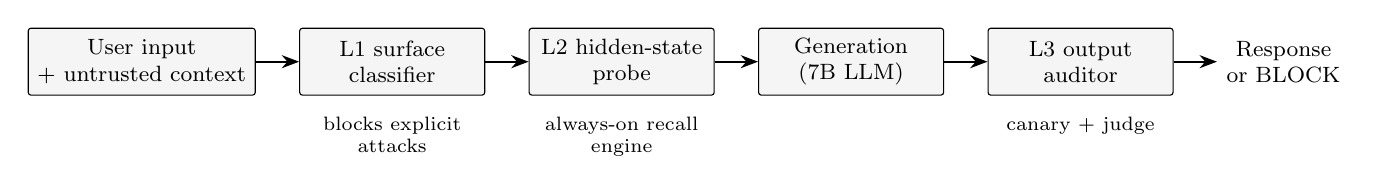
\begin{tikzpicture}[
  box/.style={draw, rounded corners=1pt, align=center, minimum height=0.85cm,
              minimum width=2.35cm, font=\footnotesize, fill=gray!8},
  arr/.style={-{Stealth[length=2.2mm]}, thick},
  node distance=0.55cm
]
\node[box] (in) {User input\\ + untrusted context};
\node[box, right=of in] (l1) {L1 surface\\ classifier};
\node[box, right=of l1] (l2) {L2 hidden-state\\ probe};
\node[box, right=of l2] (gen) {Generation\\ (7B LLM)};
\node[box, right=of gen] (l3) {L3 output\\ auditor};
\node[right=of l3, font=\footnotesize, align=center] (out) {Response\\ or BLOCK};
\draw[arr] (in) -- (l1);
\draw[arr] (l1) -- (l2);
\draw[arr] (l2) -- (gen);
\draw[arr] (gen) -- (l3);
\draw[arr] (l3) -- (out);
\node[below=0.15cm of l1, font=\scriptsize, align=center] (n1) {blocks explicit\\ attacks};
\node[below=0.15cm of l2, font=\scriptsize, align=center] (n2) {always-on recall\\ engine};
\node[below=0.15cm of l3, font=\scriptsize, align=center] (n3) {canary + judge};
\end{tikzpicture}
\caption{The three-layer pipeline. L2 runs on every input L1 does not hard-block
(``always-on'' routing); L3 audits the generated output. Any layer can block the
request, fail-closed.}
\label{fig:pipeline}
\end{figure}

\subsection{Layer 1 --- surface classifier}
\label{sec:l1}
L1 audits raw text with the ProtectAI
DeBERTa-v3-base-prompt-injection-v2 classifier \cite{he2023}. Inputs longer than the encoder window are split into
overlapping sliding windows with two production guards: an \emph{overlap clamp}
(overlap capped at a quarter of the window budget) and a \emph{window cap}
(at most $64$ windows, always including the document tail), so a long RAG
document cannot silently hide an attack or explode into hundreds of classifier
calls. A single-window input is labeled \textsc{Injection} at probability
$\ge 0.5$; a multi-window input requires either $\ge 2$ alert windows or a
peak $\ge 0.95$, so one quoted attack inside a long benign document escalates
rather than blocks. An optional ensemble (e.g., adding PIGuard
\cite{li2025}) votes per window, diluting single-model quirks such as
repetition-triggered false spikes.

\subsection{Layer 2 --- hidden-state probe}
\label{sec:l2}
L2 is a low-capacity logistic regression trained on the intermediate
activations of the \emph{target} LLM. For Qwen2.5-7B-Instruct ($28$ layers) we
extract the last-token hidden state of layer $20$ (mid-late), standardize it,
and score it with an L2-regularized logistic regression ($C{=}0.5$, balanced
class weights). The decision threshold is calibrated to an explicit
false-positive-rate (FPR) budget ($\le 1\%$) using \emph{out-of-fold}
probabilities, so it matches production scoring rather than an optimistic
in-sample ROC curve. A v2 extension concatenates pooled vectors from multiple
layers ($12,16,20,24$). The saved artifact carries a model/layer fingerprint and
\emph{refuses to load} on any model or layer mismatch, so a stale probe cannot
silently disable the layer.

\subsection{Layer 3 --- output auditor}
\label{sec:l3}
L3 audits the generated response. A cryptographically random \emph{canary}
token is embedded in the system prompt and its appearance in the output is
treated as system-prompt exfiltration; structural regex heuristics flag
compromise phrasing; and a hardened \emph{self-judge} re-examines flagged
outputs. The self-judge reuses the already-loaded target LLM (flat VRAM, no
second model to OOM), frames the audited text explicitly as data rather than
instructions, and parses only the first verdict token so a compromised response
cannot suffix-flip the decision.

\subsection{Deployment constraints}
\label{sec:deploy}
The system targets two 16\,GiB T4 GPUs (Turing, compute capability 7.5): fp16
is forced (bf16 would emulate in software), the 7B model is sharded with
\texttt{device\_map=auto} and per-GPU memory caps, the surface classifier is
pinned to GPU~1, and expandable CUDA segments avoid fragmentation OOMs. The
design reuses the single loaded 7B for generation \emph{and} judging, keeping
the whole pipeline within the two-T4 budget. The marginal cost of L2 is one
extra 7B forward pass per non-blocked request (${\sim}50$--$150$~ms at
$\le$1024 tokens).

% =============================================================================
\section{Experimental Setup}
\label{sec:setup}

\subsection{Data}
\label{sec:data}
Table~\ref{tab:data} lists the corpora. The probe is trained on the
\textbf{train} split of Deepset's prompt-injections dataset
(546 rows), augmented with $527$ jailbreak positives from
jailbreak-classification and $339$ hard negatives from NotInject
\cite{li2025}---benign text deliberately stuffed with attack trigger words,
the direct data-side antidote to over-defense. All evaluation numbers in this
paper are computed on the \textbf{held-out test split} of
prompt-injections ($116$ rows: $60$ injections, $56$ benign), which is never
seen during training; ChatGPT-Jailbreak-Prompts is reserved for cross-family
recall checks.

\begin{table}[!t]
\caption{Corpora used for training and held-out evaluation.}
\label{tab:data}
\centering
\begin{tabular}{@{}l l r l@{}}
\toprule
\textbf{Corpus} & \textbf{Split} & \textbf{Rows} & \textbf{Semantics}\\
\midrule
deepset/prompt-injections & train & 546 & binary labels (203 positive)\\
deepset/prompt-injections & test & 116 & held-out (60 inj.\ / 56 benign)\\
jailbreak-classification & train & 527 pos.\ & labeled via \texttt{type} column\\
NotInject \cite{li2025} & 3 splits & 339 & benign + trigger words (hard negatives)\\
ChatGPT-Jailbreak-Prompts & train & 79 & all positive (cross-family)\\
\bottomrule
\end{tabular}
\end{table}

\subsection{Training and calibration methodology}
\label{sec:training}
Three methodological guards matter as much as the fit itself, and each was
introduced in response to a measured failure during development:

\begin{itemize}
  \item \textbf{Evasion augmentation.} Each positive is expanded with delimiter
        smuggling, a base64 payload, and up to seven surface-evasion variants
        (zero-width characters, homoglyphs, leetspeak, ROT13, HTML comments,
        fake role tags, whitespace splits); each negative is expanded with a
        ``quoted attack'' hard negative so the probe learns the instruction
        wrapper rather than keywords.
  \item \textbf{Group-aware cross-validation.} Augmented variants of one source
        row are near-duplicates. With plain stratified folds they straddled
        fold boundaries and inflated AUC toward $1.0$ (measured $0.78$ vs.\
        $0.66$ AUC on synthetic data with the same structure). Variants now
        carry a group id and \texttt{StratifiedGroupKFold} keeps each family
        inside one fold.
  \item \textbf{Out-of-fold threshold calibration.} Reading the FPR budget off
        an in-sample ROC curve selected a threshold stricter than the budget
        actually allows ($0.9981$ vs.\ $0.9714$ in one run), silently costing
        recall. The threshold is now the largest value whose
        \emph{out-of-fold} FPR stays within the budget.
\end{itemize}

\subsection{Evaluation protocol}
\label{sec:eval}
We report true-positive rate (TPR; recall on the $60$ held-out injections),
FPR (fraction of the $56$ benign rows blocked), accuracy, and ROC-AUC. Two
gate policies are compared in one pass over the held-out set:
\textbf{Policy A (legacy gate)} blocks iff L1 hard-blocks \emph{or}
($\text{L1 score} \ge \tau_{\text{gate}}$ \emph{and} $\text{L2} \ge$ threshold),
with $\tau_{\text{gate}} = 0.30$; \textbf{Policy B (always-on)} blocks iff L1
hard-blocks \emph{or} $\text{L2} \ge$ threshold. Because the test split is
small, we emphasize that FPR has a granularity of $1/56 \approx 1.8\%$ per row
and we report counts alongside rates; bootstrap confidence intervals are
available in the released benchmark harness.

% =============================================================================
\section{Results}
\label{sec:results}

\subsection{Layers measured in isolation}
\label{sec:isolated}
Measured independently, the two input layers look like a healthy complement.
L1 (the surface classifier) alone blocks $21/60$ injections (TPR $0.350$) with
zero false positives---it catches explicit instructions but is blind to the
obfuscated and implicit ones. The L2 hidden-state probe, scored on every row
without gating, attains ROC-AUC $0.997$, TPR $0.783$ at its calibrated
threshold, and FPR $0.000$. The layers are complementary: of the $39$
injections L1 misses, the probe sees most of them clearly. On component metrics
alone, adding L2 to L1 should be a large win.

\subsection{The routing pathology}
\label{sec:pathology}
It is not. Table~\ref{tab:gate} reports end-to-end behavior. Under Policy A,
only $1$ of $60$ injections ever reaches L2: $21$ are hard-blocked by L1
(which is fine), but $38$ score below $0.30$ at L1 and are silently dropped
before the probe can see them. The probe---$0.997$ AUC in isolation---contributes
a single detection, and the ensemble recall ($0.367$) is indistinguishable from
L1 alone ($0.350$). Lowering or raising L1's block threshold does not help: the
$35$ missed injections that score below $0.01$ at L1 are simply not in the
gate's forward set, whatever the threshold.

\begin{table}[!t]
\caption{End-to-end gate-policy comparison on the held-out test split
($60$ injections, $56$ benign).}
\label{tab:gate}
\centering
\begin{tabular}{@{}l c c c c@{}}
\toprule
\textbf{Configuration} & \textbf{L2 shown} & \textbf{TPR} & \textbf{FPR} & \textbf{Acc.}\\
\midrule
L1 only & --- & 0.350 (21/60) & 0.000 & 0.664\\
Legacy gate ($\tau{=}0.30$) & 1/60 & 0.367 (22/60) & 0.000 & 0.672\\
Always-on, $\tau_{\text{L2}}{=}0.9868$ & 39/60 & 0.833 (50/60) & 0.000 (0/56) & 0.914\\
\textbf{Always-on, $\tau_{\text{L2}}{=}0.90$} & 39/60 & \textbf{0.900 (54/60)} & \textbf{0.018 (1/56)} & \textbf{0.940}\\
\bottomrule
\end{tabular}
\end{table}

Making L2 always-on (Policy B) removes the gate and lets the probe see every
input L1 does not hard-block. At the artifact's FPR-budgeted threshold
($0.9868$), end-to-end recall jumps to $0.833$ at zero measured FPR; at the
deployed operating point ($0.90$) it reaches $0.900$ at $1.8\%$ FPR. L2 now
contributes $29$ detections beyond L1's $21$ ($50$ union). The same signature
reproduces on an independent CPU stand-in (SmolLM2-135M with a probe trained on
its layer~20): recall $0.44$ under the legacy gate versus $0.67$ always-on,
with L2 adding $0$ versus $2$ detections beyond L1.

\subsection{Operating point}
\label{sec:opoint}
Table~\ref{tab:sweep} sweeps the probe threshold under always-on routing. FPR
is flat ($1/56$) from $0.50$ to $0.95$ because only one benign row ever scores
above $0.5$ on this split; on broader traffic lower thresholds will cost more
false positives. We deploy $0.90$ as the balanced point; practitioners whose
objective is maximum recall may prefer $0.75$--$0.50$.

\begin{table}[!t]
\caption{Threshold sweep under always-on routing (held-out split).}
\label{tab:sweep}
\centering
\begin{tabular}{@{}l c c c@{}}
\toprule
$\tau_{\text{L2}}$ & \textbf{TPR} & \textbf{FPR} & \textbf{Acc.}\\
\midrule
0.9868 (artifact) & 0.833 (50/60) & 0.000 (0/56) & 0.914\\
0.95 & 0.900 (54/60) & 0.018 (1/56) & 0.940\\
0.90 (deployed) & 0.900 (54/60) & 0.018 (1/56) & 0.940\\
0.75 & 0.933 (56/60) & 0.018 (1/56) & 0.957\\
0.50 & 0.950 (57/60) & 0.018 (1/56) & 0.966\\
\bottomrule
\end{tabular}
\end{table}

\subsection{Cost of the fix}
\label{sec:cost}
Always-on routing costs one additional 7B forward pass per non-blocked request
(${\sim}50$--$150$~ms at $\le$1024 tokens on two T4s). VRAM stays flat: L3
reuses the loaded target model for judging, so no second model is introduced.
For applications where that latency is unacceptable, the legacy gate can be
retained---but operators should know that on our data it reduces L2's
contribution to approximately nothing.

% =============================================================================
\section{Discussion}
\label{sec:discussion}

\subsection{Why component metrics do not compose}
\label{sec:compose}
Let $R_1$ be L1's recall, and let $G$ be the set of injections the gate
forwards to L2. If L2 achieves recall $R_2$ on $G$, end-to-end recall is
\begin{equation}
R \;=\; R_1 + (1 - R_1)\cdot g \cdot R_2,
\label{eq:recall}
\end{equation}
where $g = \Pr(\text{input} \in G \mid \text{injection, not blocked by L1})$
is the gate's coverage of L1's \emph{misses}. When the gate forwards only
inputs the surface classifier already finds suspicious, $g$ is determined by
L1's blind spots, not by L2's quality. In our legacy configuration
$g = 1/39 \approx 0.026$, so $R \approx R_1$ regardless of $R_2$---a probe
with $0.997$ AUC contributes a single catch because the gate inherits exactly
the inputs L1 cannot see. Equation~(\ref{eq:recall}) is the cascade-recall
bound in disguise \cite{viola2001,madras2018}: no downstream stage can detect
what a prior stage refuses to pass on.

\subsection{Threats to validity}
\label{sec:validity}
We state limitations explicitly because they bound the claims above. (i) The
headline numbers come from a single, small, dated corpus (116 held-out rows);
FPR granularity is $1.8\%$ per row, so point estimates are noisy and thresholds
$0.50$--$0.95$ are indistinguishable on this split. (ii) The deployed threshold
was selected using the test split, a mild form of test-set tuning; the released
trainer calibrates on a validation slice for a defensible setting. (iii) We do
not yet report leave-one-dataset-out generalization or adaptive adversaries
(obfuscation, paraphrasing, multi-turn), which the field increasingly requires
\cite{fomin2026,auc2026}; the released benchmark harness supports these.
(iv) The L1 choice (ProtectAI v2) is a documented over-defense liability
\cite{li2025}, and we observe its repetition-triggered false spikes ourselves;
the L1 ensemble and dual-key confirmation are mitigations, not eliminations.
(v) The L3 self-judge consumes untrusted text and is therefore itself
prompt-injectable; it is hardened (data framing, first-token parsing) but
scoped conservatively. We therefore position the contribution as a
\emph{measurement of how guardrail stacks fail}, not as a new detector.

\subsection{Recommendations}
\label{sec:recs}
Our findings translate into concrete practice. (1) \emph{Measure ensembles
end-to-end}: report per-layer metrics only as diagnostics; the number that
decides a deployment is the ensemble's recall on the full routing path.
(2) \emph{The cheap first stage must have near-total recall, or be bypassable.}
If a surface guard's recall is $0.35$, any layer gated behind it inherits a
$0.65$ ceiling it can never exceed. (3) \emph{Prefer always-on or learned
deferral} for expensive stages: the always-on policy here bought $+0.53$ recall
for ${\sim}100$~ms. (4) \emph{Calibrate thresholds on a validation slice, never
the test split, and report confidence intervals} on small sets. (5) \emph{Use
over-defense sets} (NotInject) as the FPR benchmark that decides real
deployments, since trigger-word bias is the dominant false-positive source.

% =============================================================================
\section{Conclusion}
\label{sec:conclusion}
We built and released a three-layer, fail-closed prompt-injection guard for
Qwen2.5-7B-Instruct on two T4 GPUs and evaluated it end-to-end. The central,
quantified finding is that a hidden-state probe with $0.997$ ROC-AUC contributed
a single detection when placed behind a conventional escalation gate, because
the gate inherited the surface classifier's blind spots and starved the probe
of $38$ of $60$ held-out injections. Making the second layer always-on raised
end-to-end recall from $0.37$ to $0.90$ at $1.8\%$ FPR. The lesson generalizes:
in layered LLM guardrails, the \emph{routing policy} between layers is a
first-class security variable, and component metrics do not predict ensemble
security. We hope the released pipeline and its failure analysis help
practitioners avoid the silent, component-metrics-driven false confidence we
measured.

% =============================================================================
% References (IEEE numbered style)
% =============================================================================
\begin{thebibliography}{99}
\bibitem{perez2022}
F. Perez and I. Ribeiro, ``Ignore previous prompt: Attack techniques for
language models,'' in \emph{Proc. NeurIPS ML Safety Workshop}, 2022,
doi: 10.48550/arXiv.2211.09527.

\bibitem{greshake2023}
K. Greshake, S. Abdelnabi, S. Mishra, C. Endres, T. Holz, and M. Fritz,
``Not what you've signed up for: Compromising real-world LLM-integrated
applications with indirect prompt injection,'' in \emph{Proc. 16th ACM
Workshop on Artificial Intelligence and Security (AISec)}, 2023, pp. 79--90,
doi: 10.1145/3605764.3623985.

\bibitem{liu2024}
Y. Liu, G. Deng, Y. Li, K. Wang, Z. Wang, X. Wang, T. Zhang, Y. Liu, H. Wang,
Y. Zheng, and Y. Liu, ``Prompt injection attack against LLM-integrated
applications,'' arXiv preprint, 2024, doi: 10.48550/arXiv.2306.05499.

\bibitem{zou2023}
A. Zou, Z. Wang, N. Carlini, M. Nasr, J. Z. Kolter, and M. Fredrikson,
``Universal and transferable adversarial attacks on aligned language models,''
arXiv preprint, 2023, doi: 10.48550/arXiv.2307.15043.

\bibitem{inan2023}
H. Inan, K. Upasani, J. Chi, R. Rungta, K. Iyer, Y. Mao, M. Tontchev, Q. Hu,
B. Fuller, D. Testuggine, and M. Khabsa, ``Llama Guard: LLM-based input-output
safeguard for human-AI conversations,'' arXiv preprint, 2023,
doi: 10.48550/arXiv.2312.06674.

\bibitem{li2025}
H. Li, X. Liu, N. Zhang, and C. Xiao, ``PIGuard: Prompt injection guardrail
via mitigating overdefense for free,'' in \emph{Proc. 63rd Annual Meeting of
the Association for Computational Linguistics (ACL)}, 2025, pp. 30420--30437,
doi: 10.18653/v1/2025.acl-long.1468.

\bibitem{injecguard}
H. Li, X. Liu, and C. Xiao, ``InjecGuard: Benchmarking and mitigating
over-defense in prompt injection guardrail models,'' arXiv preprint, 2024,
doi: 10.48550/arXiv.2410.22770.

\bibitem{instructdetector}
T. Wen, C. Wang, X. Yang, H. Tang, Y. Xie, L. Lyu, Z. Dou, and F. Wu,
``Defending against indirect prompt injection by instruction detection,'' in
\emph{Findings of the Association for Computational Linguistics: EMNLP 2025},
2025, pp. 19472--19487, doi: 10.18653/v1/2025.findings-emnlp.1060.

\bibitem{jbshield}
S. Zhang, Y. Zhai, K. Guo, H. Hu, S. Guo, Z. Fang, L. Zhao, C. Shen, C. Wang,
and Q. Wang, ``JBShield: Defending large language models from jailbreak attacks
through activated concept analysis and manipulation,'' in \emph{Proc. USENIX
Security Symposium}, 2025, doi: 10.48550/arXiv.2502.07557.

\bibitem{fomin2026}
M. Fomin, ``When benchmarks lie: Evaluating malicious prompt classifiers under
true distribution shift,'' arXiv preprint, 2026,
doi: 10.48550/arXiv.2602.14161.

\bibitem{auc2026}
Y. Li, Z. Fan, and Z. Zhuang, ``When AUC 0.998 is not enough: A candidate
evaluation protocol for hidden-state probes of indirect prompt injection in
multimodal computer-use agents,'' arXiv preprint, 2026,
doi: 10.48550/arXiv.2606.22864.

\bibitem{alain2016}
G. Alain and Y. Bengio, ``Understanding intermediate layers using linear
classifier probes,'' in \emph{Proc. ICLR Workshop Track}, 2017,
doi: 10.48550/arXiv.1610.01644.

\bibitem{viola2001}
P. Viola and M. Jones, ``Rapid object detection using a boosted cascade of
simple features,'' in \emph{Proc. IEEE Conf. Computer Vision and Pattern
Recognition (CVPR)}, 2001, pp. I-511--I-518, doi: 10.1109/CVPR.2001.990517.

\bibitem{madras2018}
D. Madras, T. Pitassi, and R. Zemel, ``Predict responsibly: Improving fairness
and accuracy by learning to defer,'' in \emph{Proc. Advances in Neural
Information Processing Systems (NeurIPS)}, 2018,
doi: 10.48550/arXiv.1711.06664.

\bibitem{he2023}
P. He, J. Gao, and W. Chen, ``DeBERTaV3: Improving DeBERTa using
ELECTRA-style pre-training with gradient-disentangled embedding sharing,'' in
\emph{Proc. International Conference on Learning Representations (ICLR)}, 2023,
doi: 10.48550/arXiv.2111.09543.

\bibitem{qwen25}
Qwen Team, Alibaba Group, ``Qwen2.5 technical report,'' arXiv preprint, 2024,
doi: 10.48550/arXiv.2412.15115.
\end{thebibliography}

\end{document}
